% Trying to break the document up a bit.  This command simply inserts the contents of the file at this point.  It contains the document license, preamble, and title page: things that aren't likely to change more than once.  This can be used to separate discrete parts of a document into files that are easier to edit at one time.
%%%%%%%%%%%%%%%%%%%%%%%%%%%%%%%%%%%%%%%%%%%%%%%%%%%%%%%%%%%%%%%%%%%%%%
% This layout was adapted from one found at latextemplates.com which
% was adapted from another.
%
% License: CC BY-NC-SA 3.0
% (http://creativecommons.org/licenses/by-nc-sa/3.0/)
%
% Original header:
%
% This is a LaTeX version of the sample laboratory report from
% Virginia Tech's copyrighted 08-09 CHEM 1045/1046 lab manual.
% Reproduction of this one appendix section for academic purposes
% should fall under fair use.
%
%%%%%%%%%%%%%%%%%%%%%%%%%%%%%%%%%%%%%%%%%%%%%%%%%%%%%%%%%%%%%%%%%%%%%%

\documentclass{article}

\usepackage{graphicx}
% \usepackage[acronym]{glossaries} % Lets us use acronyms
\usepackage{multicol}
\usepackage{amsmath}
\usepackage{siunitx} % SI units in math mode
%\usepackage[usenames]{color}
\usepackage{subcaption}

\author{}
\title{ELEC-313 \\ Lab 9: Common-Emitter Transistor Amplifier\\ }
\date{\today}

% \loadglsentries{acronyms} % Actually loads 'acronyms.tex'
% \makeglossaries

\begin{document}

\maketitle

\begin{center}
  \begin{tabular}{lr}
    Date Performed: & November 20, 2013 \\
    Partners:       & Charles Pittman    \\
    & Stephen Wilson     \\
  \end{tabular}
\end{center}

\newpage

%\tableofcontents
%\listoffigures
%\listoftables
%\newpage

% Number the enumerate environment (unordered lists) by letter:
% \renewcommand{\labelenumi}{\alph{enumi}.}

\section{Objective}

The objective is to construct and observe the operation of a common-emitter transistor amplifier.

\section{Equipment}

\begin{tabular}{ll}
  \centering
  Transistor: 2N2222A & Capacitor: \SI{0.1}{\micro\farad} \\
  Resistors: \SI{100}{\kilo\ohm}, \SI{20}{\kilo\ohm}, \SI{1}{\kilo\ohm}, \SI{470}{\ohm} & Power supply: HP E3631A \\
  Function generator: HP 33120 & Oscilloscope: Agilent 54622D \\
  \multicolumn{2}{l}{Multimeters: HP 34401A, Fluke 8010A (x2)} \\
\end{tabular}

\section{Schematics}

\begin{figure}[hbtp]
  \centering
  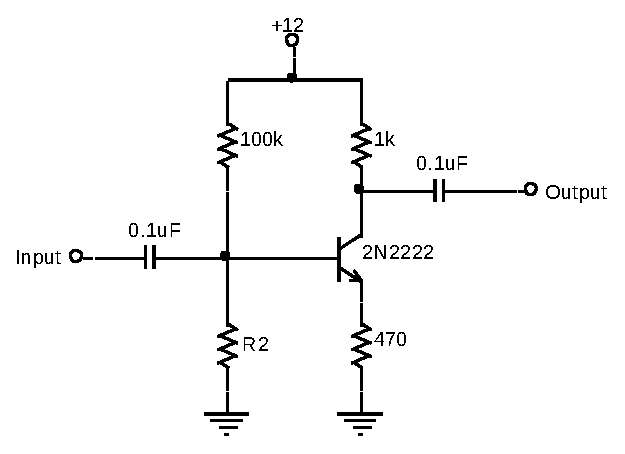
\includegraphics[width=.7\textwidth]{circuit}
  \caption{\label{fig:circuit} Common-emitter transistor amplifier (without the emitter bypass capacitor). $R_2$ = \SI{20}{\kilo\ohm}}
\end{figure}

\section{Procedure}
The following procedure was used to evaluate the transistor amplifier of Figure~\ref{fig:circuit}:

\begin{enumerate}
\item The circuit of Figure~\ref{fig:circuit} was constructed.
\item The DC voltage at each terminal of the transistor was measured and the values were recorded in Table~\ref{tab:amp}.
\item The output of the function generator was connected to the input of the circuit. Then the function generator was set to a frequency of \SI{30}{\kilo\hertz} as a sine wave.
\item Channel 1 of the oscilloscope was connected to the input of the circuit and channel 2 connected to the output.
\item The amplitude of the sinusoidal waveform was adjusted to -\SI{250}{mV} to +\SI{250}{mV} (\SI{500}{mVpp}) at the circuit input as measured on the oscilloscope.
\item The peak-to-peak amplitude of the output waveform ($V_o$) was measured and recorded in Table~\ref{tab:amp}.
\item Then the voltage gain ($A_V$) of the amplifier was computed and recorded in Table~\ref{tab:amp}.
\item The decade resistance box was connected to the output of the circuit and adjusted until the output voltage read as one-half the open circuit value measured in step 6. The displayed resistance value, which is also equivalent to the output resistance ($R_o$) of the circuit, was recorded in Table~\ref{tab:imp}.
\item The function generator was disconnected from the circuit input and then connected to the oscilloscope to measure the open circuit voltage ($V_{OC}$) produced by the generator. The open-circuit voltage was recorded in Table~\ref{tab:imp}.
\item The decade box was removed from the output and reconnected between the function generator and the open circuit input, so that the signal travels from the function generator and through the resistance box on its way to the circuit input.
\item The decade resistance box was adjusted so that the voltage measured at the circuit input is one-half the open circuit voltage measured in step 9. That displayed resistance is \SI{50}{\ohm} less than the input resistance ($R_i$) of the circuit. The input resistance was recorded in Table~\ref{tab:lrg_sig}.
\item The decade resistance box was removed and the function generator was reconnected directly to the circuit input, and its frequency was left at \SI{30}{\kilo\hertz}.
\item The amplitude of the generator was slowly increased while the output waveform was carefully observed to determine the point at which the output waveform began to clip ($V_{clip}$). The peak-to-peak voltage was recorded in Table~\ref{tab:lrg_sig}.
\item The \SI{10}{\micro\farad} emitter bypass capacitor was inserted into the circuit.
\item Steps 2 through 7 were repeated, except the input voltage was first reduced until the waveform didn’t clip, and values recorded in Table~\ref{tab:amp_bypass}
\end{enumerate}

\section{Results}

\begin{table}[hbtp]
  \centering
  \begin{tabular}{ccc|cc|c}
    $V_B$    & $V_C$    & $V_E$    & $V_i$     & $V_o$     & $A_V$ \\
    (\si{V}) & (\si{V}) & (\si{V}) & (\si{mV}) & (\si{mV}) &       \\
    \hline
    1.788    & 9.58     & 1.153    & 500       & 970       & 1.94  \\
  \end{tabular}
  \caption{\label{tab:amp} Transistor amplifier characteristics}
\end{table}

\begin{table}[hbtp]
  \centering
  \begin{tabular}{cc}
    $R$         & $V_{OC}$  \\
    (\si{\ohm}) & (\si{mV}) \\
    \hline
    958         & 477       \\
  \end{tabular}
  \caption{\label{tab:imp} Port impedances}
\end{table}

\begin{table}[hbtp]
  \centering
  \begin{tabular}{cc}
    $R$              & $V_i$    \\
    (\si{\kilo\ohm}) & (\si{V}) \\
    \hline
    13.9             & 2.57     \\
  \end{tabular}
  \caption{\label{tab:lrg_sig} Large-signal performance}
\end{table}

\begin{table}[hbtp]
  \centering
  \begin{tabular}{ccc|cc|c}
    $V_B$    & $V_C$    & $V_E$    & $V_i$    & $V_o$    & $A_V$ \\
    (\si{V}) & (\si{V}) & (\si{V}) & (\si{V}) & (\si{V}) &       \\
    \hline
    1.783    & 9.547    & 1.164    & 0.122    & 6.19     & 52.0
  \end{tabular}
  \caption{\label{tab:amp_bypass} Transistor amplifier characteristics (with emitter bypass capacitor)}
\end{table}

\begin{table}[hbtp]
  \centering
  \begin{tabular}{c|ccc}
    & Measured & Calculated & \% Diff. \\
    \hline
    $R_o$ & \SI{958}{\ohm} & \SI{1}{\kilo\ohm} & 4.20\% \\
    $R_i$ & \SI{13.95}{\kilo\ohm} & \SI{13.543}{\kilo\ohm} & 3.01\% \\
    $A_V$ (no bypass) & -1.94 & -2.06 & 5.83\$ \\
    $A_V$ (with bypass) & -50.9 & -111 & 54.14\% \\
  \end{tabular}
  \caption{\label{tab:gains} Percent differences}
\end{table}

\newpage

\section{Conclusion}
\label{sec:conclusion}

As seen in Table~\ref{tab:amp_bypass}, the small signal voltage gain $A_V$ increased once the emitter bypass capacitor was added, even though it had relatively insignificant impact to the DC voltages of each terminal. The DC voltages shouldn’t change because the capacitor that was added is ideally an open circuit. But the emitter bypass resistor has a significant impact to the AC analysis because it is seen as a closed circuit and allows the $I_E$ to pass through. As seen in Eq~\ref{eq:gm2}, the addition of the emitter bypass capacitor, reduced the denominator of the $A_V$ Eq~\ref{eq:Av1}, thus increasing gain.

Table~\ref{tab:gains} shows the percent differences of the small signal gains along with input and output impedances ($R_i$ and $R_o$) both with and without the bypass capacitor. The 5.7 percent difference between the $A_V$ (no bypass) is caused from a combination of using nominal instead of measured resistance values, and the assumptions that $\beta$ was assumed to be 150 and  $I_{CQ}$ was assumed to be \SI{3}{mA} (from the pre-lab). $I_{CQ}$ was probably less than \SI{3}{mA} because the voltage drop between the \SI{12}{VDC} input and terminal C is smaller. There is significant percent difference between the theoretical $A_V$ versus the measured $A_V$ with the bypass emitter. Eq~\ref{eq:gm2} shows that the calculated $A_V$ is affected more by $I_{CQ}$. Also, when calculating the theoretical votage gain, $r_o$ is assumed to be infinite (i.e. an open circuit), which is not entirely true. %<Not sure what you were saying>The resistance of $r_o$ in parallel with $R_C$ this would actually have been slightly less than the $R_o$ used in the theoretical calculations.

%$R_i$ and $R_o$ are relatively close and the small percent differences are probably because we took the nominal resistor values instead of the measured resistor values. Experience has shown that resistors are usually slightly less than their nominal value.
% Table~\ref{tab:gains} shows the $V_{OC}$ recorded during step 9. It is less than \SI{500}{mV} probably because of “noise” could have affected the output reading. The table also shows the $V_{clip}$, which is the point at which the output voltage began to clip (when the transistor is at saturation).

\section{Equations}

% LaTeX sees blank lines as a start of another paragraph.  To avoid
% unnecessary vertical spaces between equations, and still visually
% separate in source, put a comment between them.
%
\begin{equation}
  \label{eq:Ri}
  R_i = R_1 | R_2 | R_3
\end{equation}
%
\begin{equation}
  \label{eq:Rib}
  R_{ib} = r_\pi + (1+\beta) R_E
\end{equation}
%
\begin{equation}
  \label{eq:rpi}
  r_\pi = \frac{V_T\beta}{I_{CQ}}
\end{equation}
%
\begin{equation}
  \label{eq:Av1}
  A_V = \frac{-\beta R_o}{R_{ib}} \cdot \left( \frac{R_i}{R_i + R_S} \right)
\end{equation}
%
\begin{equation}
  \label{eq:gm1}
  g_m = \frac{\beta}{r_\pi}
\end{equation}
%
\begin{equation}
  \label{eq:Av2}
  -g_mR_o \cdot \left(\frac{R_i}{R_i + R_S} \right) = \frac{I_{CQ}R_oR_i}{R_i + R_S}
\end{equation}
%
\begin{equation}
  \label{eq:gm2}
  g_m = \frac{I_{CQ}}{V_T}
\end{equation}

\end{document}
